%
% File emnlp2015.tex
%
% Contact: daniele.pighin@gmail.com
%%
%% Based on the style files for ACL-2015, which were, in turn,
%% Based on the style files for ACL-2014, which were, in turn,
%% Based on the style files for ACL-2013, which were, in turn,
%% Based on the style files for ACL-2012, which were, in turn,
%% based on the style files for ACL-2011, which were, in turn, 
%% based on the style files for ACL-2010, which were, in turn, 
%% based on the style files for ACL-IJCNLP-2009, which were, in turn,
%% based on the style files for EACL-2009 and IJCNLP-2008...

%% Based on the style files for EACL 2006 by 
%%e.agirre@ehu.es or Sergi.Balari@uab.es
%% and that of ACL 08 by Joakim Nivre and Noah Smith

\documentclass[11pt,a4paper]{article}
\usepackage{acl2015}
\usepackage{times}
\usepackage{url}
\usepackage{latexsym}
\usepackage{color}
\usepackage{enumitem}
\usepackage{booktabs}
\usepackage{graphicx}
\usepackage{todonotes}


%\setlength\titlebox{5cm}

% You can expand the titlebox if you need extra space
% to show all the authors. Please do not make the titlebox
% smaller than 5cm (the original size); we will check this
% in the camera-ready version and ask you to change it back.


\title{Profiling word-sense agreement variation}

\author{First Author \\
  Affiliation / Address line 1 \\
  Affiliation / Address line 2 \\
  Affiliation / Address line 3 \\
  {\tt email@domain} \\\And
  Second Author \\
  Affiliation / Address line 1 \\
  Affiliation / Address line 2 \\
  Affiliation / Address line 3 \\
  {\tt email@domain} \\}

\date{}

\begin{document}
\maketitle
\begin{abstract}
\section{Introduction}

Some of the disagreement on sense annotation is systematic, and is a result of the interplay between the linguistic properties of the examples and the characteristics of the sense inventory. We propose a regression method to predict systematic disagreement, namely the variation of agreement in sense-annotated examples that depends on the linguistic features of the headword and its contexts.
 In this article we tackle the estimation of the likely agreement of a sense-annotated example by means of regression. \textcolor{red}{ We observe so and so}. 
\end{abstract}

\cite{Artstein2008} provide interpretation of Kripperdorff's $\alpha$ coefficient to describe the reliability of an annotation task, and the way that observed agreement ($A_o$) is calculated for each example. We describe a method to predict the $A_o$ of the examples in our datasets. 

\cite{krippendorff2011} defines disagreement as \textit{by chance}---caused by unavoidable inconsistencies in annotator behavior---and \textit{systematic}---caused by properties of the data being annotated. We know some of the difficult examples in our dataset to have lower agreement, which can be a result of the linguistic characteristics of these examples.

Even though, strictly speaking, the value of $\alpha$ only provides an indication of the replicability of an annotation task, we suggest that the difficulty of annotating a particular example will influence its local observed agreement. Thus, easy examples will have a high $A_o$, that will drop as difficulty increases. 

Identifying low-agreement examples by their linguistic features would help characterize contexts that make words difficult to annotate.


The goal of this experiment is to measure how much of the disagreement in the annotations is caused by linguistic properties of the examples and is thus systematic. More specifically, we intend to interpret the $R^2$ determination coefficient of a regression model on the linguistic features.1

We will consider the proportion of explained variance of the regression model described by the coefficient of determination $R^2$ to be the amount of disagreement our system can give account for, and is thus systematic. 

\paragraph{Contributions} \textcolor{red}{This and that}.

\section{Related work}


\cite{Plank2014} 

\cite{Jurgens2014}

\cite{Passonneau2014}

\cite{Jurgens2013}

\cite{Lopez2015} study the agreement-to-performance correlation for WSD. \\

Disagreement between annotators is commonly seen as some kind of featureless noise. However, there are authors that take the stance that, when an item is annotated with low-agreement and the labels it gets assigned are disparate, there is a case for seeing this particular example as difficult to annotate. One of the causes for this difficulty can be regular polysemy.

\cite{Tomuro2001a} provides an interpretation on disagreement between sense-annotated corpora. Her hypothesis is that, when humans disagree on senses of a word, there is an underlying relation between the senses, that is, most inter-annotator disagreement is explained by systematic polysemy. 

Tomuro compares the sense annotations of two corpora, SemCor and DSO, and reports an average K between the sense annotations of the two corpora in their matching sentences of 0.264. She concedes however that a good proportion of the difference is a result of SemCor being annotated by lexicographers and DSO by novices, but claims that these differences provide insight on sense distinctions that are easily misjudged. She is also careful to note that the inverse of her hypothesis does not work, and that systematic polysemy does not cause disagreement per se.  \cite{Jezek2010} also remark that the nouns that cause most disagreement in the coercion annotation task are precisely dot objects.


\section{Method}

Observed agreement $A_o$ is a continuous variable, and using supervised learning to predict it from the linguistic features in Chapter \ref{chap:feats} is a regression task, similar to the regression task to predict literality in Chapter \ref{chap:wsd}

For each dataset $D$, we generate a dataset $D_{agr}$ where the sense annotations are replaced by the observed agreement $A_o$ of each example. Note that the $\alpha$ coefficient is an aggregate measure that is obtained dataset-wise, and $A_o$ is the only agreement measure available for each individual example.

The method for agreement prediction is the same as in literality prediction (cf. Section \ref{sec:reglit_method}), with the exception of the dependent variable. We use the \textsc{all} feature set as explanatory variables. It is still a class-based method because we are not looking at the identity of the headword for training. 

We train and test on Bayesian Ridge regression using  $10\times10$ CV.

\subsection{Target variable resolution}
A smoother target variable is easier to fit. Fewer annotators per item yield more jagger distributions of $A_o$, with fewer different intermediate values. The higher the amount of annotators, the better the resolution of the target variable. 

\section{Data}
We use the following datasets, available with more than two annotations per item. When a dataset has been doubly annotated and then adjudicated, we treat the adjudication as a third annotation.
\todo[inline]{1) Come up with good acronyms for the datasets}
\todo[inline]{2) It could be sufficient to do it only for the English data. Time- and results-permiting it would be great to incorporate more languages}


English\\
\begin{enumerate}[noitemsep]
\item MASC \cite{Passonneau2012} crowdsourced 
\item MASC word-sense corpus annotated by experts \cite{Passenau2010}
\item The FrameNet data of \cite{Sogaard2015}. We use the frame-name layer as a word-sense layer, taking the frame-evoking word as headword.
\item The synset-annotated data of \cite{Gella2014}.
\item The regular polysemy dataset of \cite{MartinezAlonso2013}
\item The superse-annotated dataset of \cite{Johannsen2014}
\end{enumerate}



Non-English
\begin{enumerate}[noitemsep]
\item The regular polysemy dataset of \cite{MartinezAlonso2013} for Spanish and Danish
\item The superse-annotated dataset of \cite{MartinezAlonso2015} for Danish
\item EusemCor 
\end{enumerate}

\begin{table*}[Ht!]

\begin{center}
  \begin{tabular}{ccccccc}
  \toprule 

Dataset& lang & Inventory & instances & annotators & type &alpha \\ 
\midrule 

S15 & en & FrameNet & XXX & 3 & e & xxxx \\
MASC & en & synsets & & & c & \\
J14 & en & supersenses  & & & e & \\
M13EN & en & LMU & 1500 & 3 & c&  \\
DSC & da & supersenses &    &  & c& \\
M13ES & es &  &  &  & c&  \\
M13DA & da &  &  &  & c&  \\
G14 & en &  synsets &  &  & c&  \\
\bottomrule

  \end{tabular}  
\end{center}
\caption{Datasets \label{tab:data} \textcolor{red}{This table needs filling}}
\end{table*} 

\section{Features}
We define an \textit{instance} as a sentence with a word $w$ chosen for annotation. If a sentence has $n$ annotated sentences, it yields $n$ instances. For each instance, we calculate the following features---based on \cite{Yarowsky2002}---for a word $w$ and its syntactic parent $p$. 
\begin{enumerate}[noitemsep]
\item  frequency of $w$, frequency $p$. We recast frequency as the inverse of the rank.
\item pos of $w$, pos of $p$
\item pos bigram left and right.
\item number of dependents of $w$, number of dependents of $p$, bag-of-labels for the dependents of $w$ and the dependents of $p$
\item distance to root of $w$
\item number of possible senses \todo[inline]{Maybe a better entropy-based measure?}
\item length of the sentence; length of the sentence in content words.
\item generality of $w$ (approximated by the entropy of the softmaxed embedding of $w$, cf Lazaridou.
\item sense relatedness (wordnet distance between senses, something like this) -- avg, min and max
\item sense specificity (depth in wordnet or framenet) --- avg, min and max
\item proportion of homographs for $w$ conditioned by pos tag (i.e. "change" is 0.8 noun).
\item A bag of words of the context of $w$ --- \todo[inline]{I really would prefer not use lexical features at all, it makes the system more robust across languages.}
\end{enumerate}

We use TreeTagger for part-of-speech tagging and TurboParser for dependency parsing. All tagging and parsing models are trained on the Universal Dependencies v1.1, which allows cross-language comparison of features.

\section{Results}

Table \ref{tab:regagr_results} shows the scores for agreement prediction for all nine datasets.
MSE-$ \overline{LS}$ is the MSE obtained by assigning each example with the average observed agreement ($ \overline{A_o}$),  MSE-BR is the MSE for the system using Bayesian Ridge regression, and $R^2$ is the coefficient of determination for Bayesian Ridge.
 Cf. Section \ref{sec:reglit_method} for a review of the evaluation metrics for regression.
\subsection{Model inspection}
Fitting a regression model yields a coefficient for each feature. Coefficients can be negative or positive, thus helping to decrease or increase the value of the predicted variable. We examine the coefficients for the six datasets that fit over baseline.  Appendix \ref{sec:apdx_agreement} provides the top 20  positive and top 20 negative coefficients for each dataset. We have obtained these coefficients by fitting the regression algorithm on all the 500 examples for each dataset and not by $10\times10$ CV, in order to obtain one stable ranking of features calculated at one for each dataset.  As in the previous chapters, $h$ stands for the dot-type headword of each example.

We observe that the grammatical features have positive coefficients more often than not. This indicates that explicit syntactic behavior helps the annotators take decisions that are consistent. Nevertheless, some few grammatical features correlate with a lower agreement, and we interpret them as causes of systematic disagreement. For the \textsc{locorg} datasets, we identify no grammatical features with high negative coefficients. For the \textsc{contcont} datasets, however, we identify several grammatical features that help identify systematic disagreement.

When the preposition \textit{in} is the head of $h$ for an English \textsc{contcont} word, the agreement decreases. This preposition is normally associated with literal meaning, but its presence also diminishes the agreement in examples like first English sentence in (\ref{ex:agrfeats}).

For Spanish, $h$ being complemented by a quantifier is a feature that reveals possible low agreement. This is similar to the example d) in \ref{ex:spalocorgsenses} for Spanish, but also to the Danish example d) in  \ref{ex:dacontcontsenses}. In both examples from Chapter \ref{chap:ansch} the container word is introduced by a quantifier, and the examples received minimal agreement. 
 
For Danish, container nouns in definite form have low agreement. Although noun definiteness is a matter of morphology (cf. Section \ref{sec:theory_danishspanish}
), this is an an example of systematic disagreement caused by pragmatics: the definite form is used when there is a referent that has already been mentioned previously, but the annotation has been carried out sentence-wise. Thus, many referents are not provided, and that makes the annotator's task more difficult. 

Danish also has a specific syntactic structure to indicate whether a container is used to mean a measure of unit of some substance, in which the the noun for the container and for the substance are said consecutively. Thus, ``et glas vand" (glossed as ``a glass water") means ``a glass \textit{of} water". This structure, represented in the Danish treebank as the content being a dependent of the container, is also a cause of systematic disagreement. 



\begin{table}[Ht!]

\begin{center}
  \begin{tabular}{l ccc}
 \toprule


 Dataset& MSE-$\overline{A_o}$ & MSE-BR &  $R^2$\\
 \midrule

\textsc{eng:animeat} & 0.06 & 0.06 & -0.02  \\ 
\textsc{eng:artinfo} & 0.06 & 0.05  & -0.02  \\ 
\textsc{eng:contcont} & 0.08 & \textbf{0.08}  & \textbf{0.01}\\ 
\textsc{eng:locorg} & 0.08 & \textbf{0.08}  & \textbf{0.00}\\ 
\textsc{eng:procres} & 0.06 & 0.06  & -0.03 \\ 
\textsc{da:contcont} & 0.13 & \textbf{0.13} & \textbf{0.05}\\ 
\textsc{da:locorg} & 0.13 & \textbf{0.13} & \textbf{0.01}\\ 
\textsc{spa:contcont} & 0.09 & \textbf{0.09} & \textbf{0.03}\\ 
\textsc{spa:locorg}& 0.08 & \textbf{0.07} & \textbf{0.02}\\ 
\bottomrule

  \end{tabular}  
\end{center}
\caption{Evaluation for agreement prediction \label{tab:regagr_results} \textcolor{red}{This table is a placeholder taken from my thesis, it just shows what I intend to show}}
\end{table} 

Notice there are negative values of $R^2$. This means that the system would be better approximated by disregarding all features and assigning the average $A_o$ for these three datasets. For positive values of $R^2$, we can claim that there is at least that much proportion of the disagreement that can be explained by the features and is thus systematic.

Significant (corrected paired t-test with $p < 0.05$) improvements over the $\overline{A_o}$ baseline are marked in bold. The $R^2$ scores are lower for agreement prediction than for literality prediction (cf. Table \ref{tab:reglit_results}), and the difference between MSE-$\overline{A_o}$ and MSE-BR can only be observed in the third or fourth decimal place, which do not appear in the tables. 


\begin{figure*}[htt]
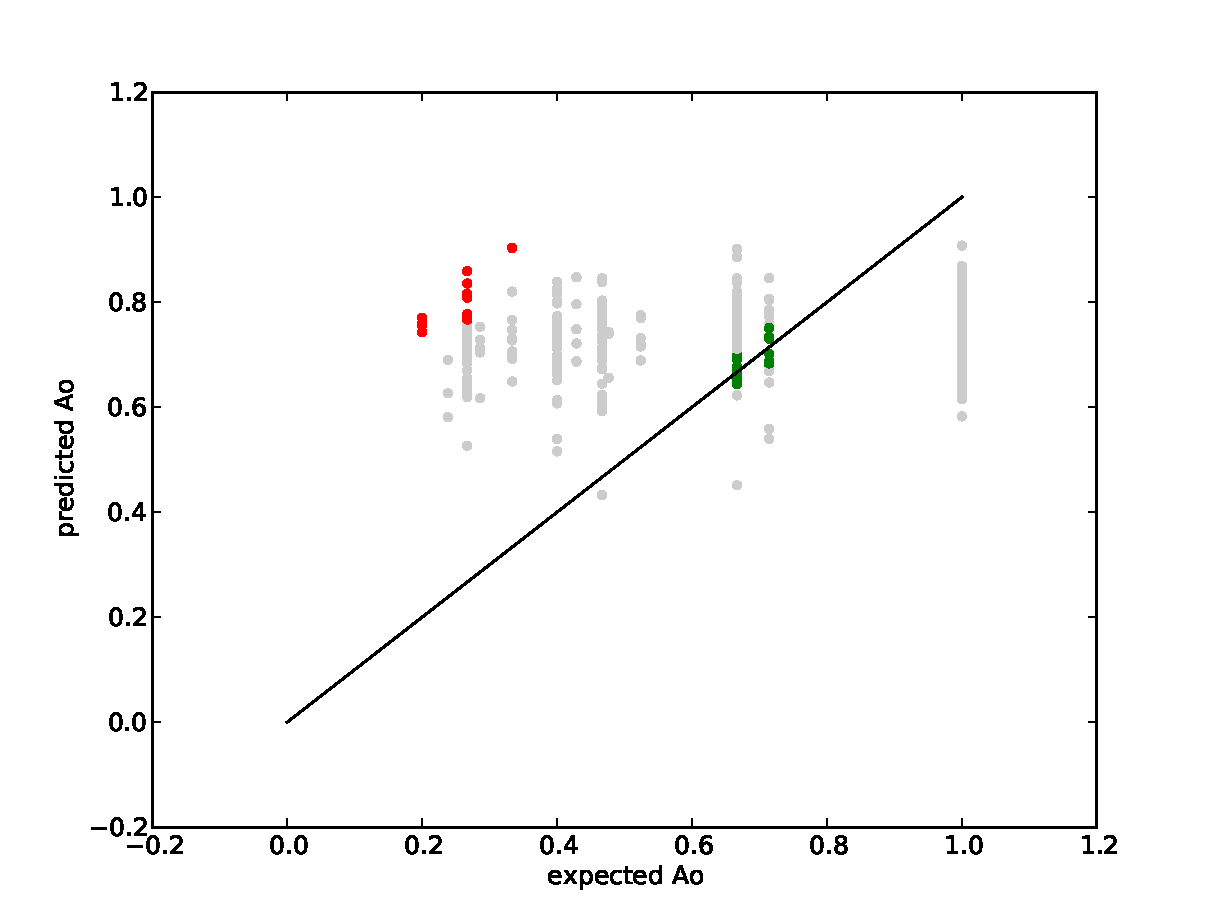
\includegraphics[scale=0.25]{scatterdraft.pdf}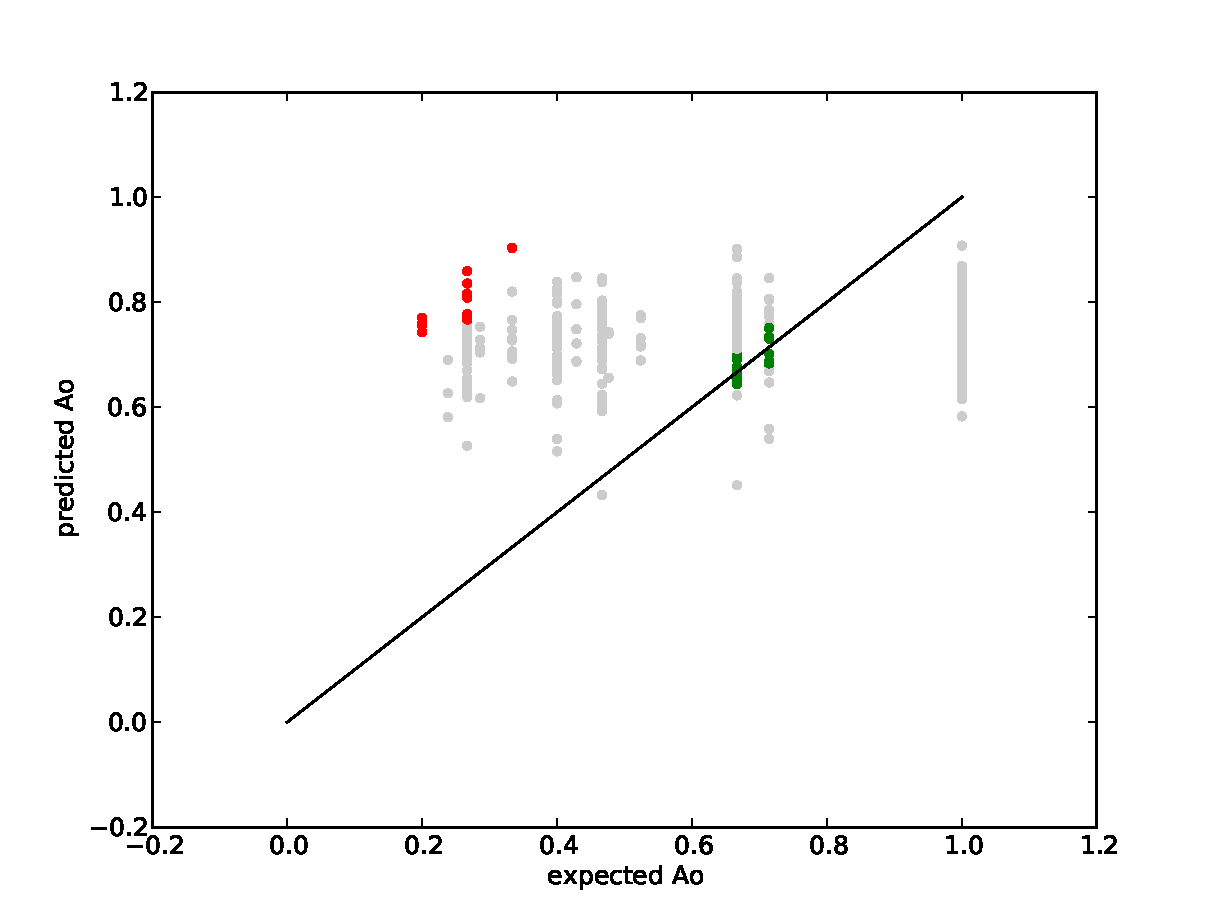
\includegraphics[scale=0.25]{scatterdraft.pdf}
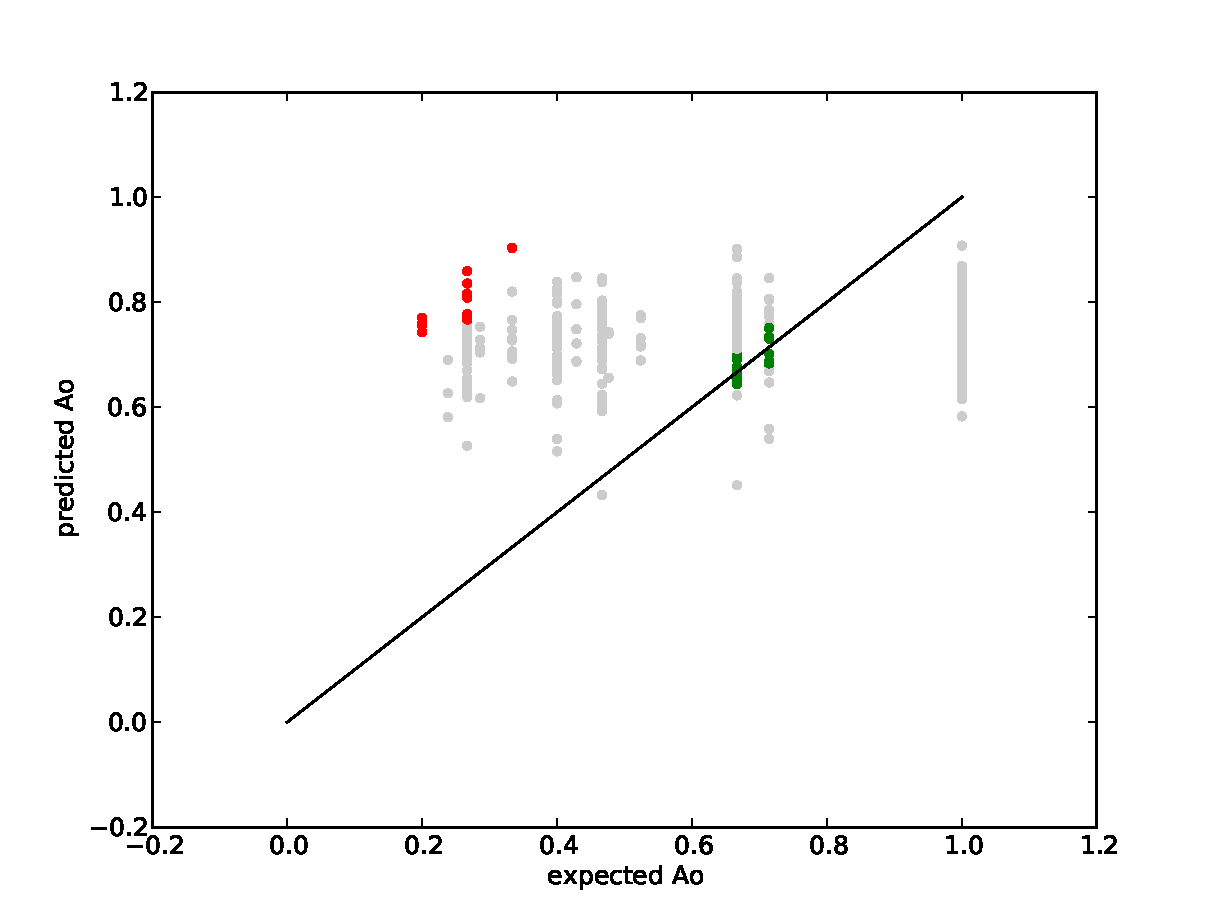
\includegraphics[scale=0.25]{scatterdraft.pdf}

\caption{ \label{fig:reglit_dklocorg}\textcolor{red}{Comparative scatterplots for some datasets}}    
\end{figure*}
The datasets that can be fit over baseline, and whose disagreement can be partially explained by the linguistic features are the datasets for \textsc{contcont} and \textsc{locorg} for all three languages. Datasets with very high or very low agreement have too little variation for the system to be able to pick on patterns that relate the features to the dependent variable. 

The Danish and Spanish datasets, annotated by volunteers, show more identifiable systematic disagreement, regardless of their $\alpha$ score. The dataset with more (5\% for an $R^2$ of 0.05) identified systematic disagreement is \textsc{da:contcont}, which has been the most difficult dataset to automatically resolve with WSD, even disregarding the underspecified sense (cf. Section \ref{sec:wsd_results}). 


% include your own bib file like this:
%\bibliographystyle{acl}
%\bibliography{acl2015}





This lack of variance can be seen in the less smooth values of $A_o$ shown in Figures \ref{fig:distagrdeng} and \ref{fig:distagrdkspa}, which are grouped in ranges.

The datasets we cannot fit over baseline are \textsc{eng:animeat}, \textsc{eng:artinfo}, and \textsc{eng:procres}. The last two datasets have fared consistently badly in the WSD experiments (cf. Section \ref{sec:wsi_eval}), and have low (0.12 and 0.10) $\alpha$ scores, besides being the two datasets with the highest difference (D) proportion in Table \ref{tab:mace}. 

The high D proportion indicates that the annotations for these two datasets are not very stable, and the low $\alpha$ indicates that repeating the annotation task with the same examples would yield very different sense annotations. The impossibility to fit the agreement prediction system over the baseline suggests, along with the previous reasons, that these two datasets have no example-wise systematic disagreement. The inability of neither finding systematic disagreement or accurately identifying the senses of these datasets by WSD indicate that the annotations are not reliable. 

The \textsc{eng:animeat} dataset, which also resists agreement prediction, is different to \textsc{eng:artinfo} and \textsc{eng:procres} in three aspects. Firstly, it has the highest $\alpha$ of all nine datasets. Secondly, it has the lowest amount of underspecified senses by either the expert or the turkers. Thirdly, it is the dataset with highest overall accuracy in WSD (cf. Section \ref{sec:wsd_results}), and the second highest in literality prediction.

However, it is not possible for the system to identify any systematic disagreement in \textsc{eng:animeat}. This is due to the low variance of the dependent variable, which makes this dataset the complementary to \textsc{eng:artinfo} and \textsc{eng:procres}: the sense distinction is arguably too easy for the annotators, and the system cannot find a mapping between the linguistic features and the little disagreement. 

\section{Conclusions}

We have described a system to predict the observed agreement $A_o$  and automatically determine examples that have low agreement. The learnability of the task is limited by the resolution of the target variable, the annotator bias (more relevant for crowdsourcing, as a result of the risk-avoiding strategy many turkers use), and the performance of the predictions for part of speech and syntactic dependencies.

Nevertheless, we have been able to fit X datasets over baseline, namely the three language variants of the \textsc{contcont} and \textsc{locorg} datasets. The datasets that cannot be fit are the two lowest-agreement datasets, and the highest-agreement dataset, which has too little variation in $A_o$ for the relation between dependent variable and features to be modelable.


\todo[inline]{If the following statement holds for all the datasets, I am a happy man.}
Most syntactic features correlate with high agreement, which implies that marked syntactic contexts help an univocal interpretation. Most negative features for agreement are lexical, which indicates that difficult or unusual words get on the way of annotator agreement.

However, we have found linguistic cues that pinpoint to syntactic behavior of the headword that cause agreement to drop, because annotators interpret them in different manners. 

%There are no features for the headword, because we are using features from the class-based WSD and the headword is abstracted away. Including the headword would improve $R^2$ because a great deal of the variation in agreement between datasets is caused by the headword and the semantic class, regardless of context. 

This system can be used as an automatic review method for sense-annotation tasks, because it identifies a proportion of systematic disagreement that can be attributed to certain linguistic features, which can lead to reviews of annotation guidelines. 



\bibliographystyle{acl}
\bibliography{biblio}

\end{document}
